\documentclass{standalone}
\usepackage{tikz}
\usetikzlibrary{patterns}

\begin{document}
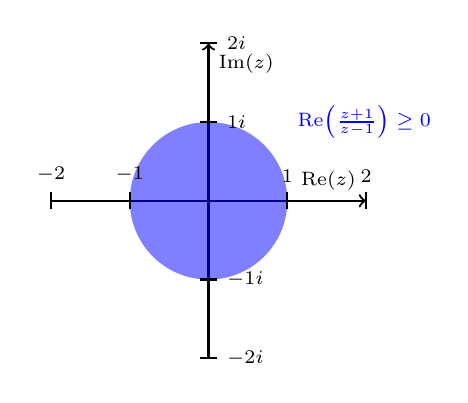
\begin{tikzpicture}
    \begin{scope}[thick,font=\scriptsize]

        \draw [->] (-2,0) -- (2,0) node [above left]  {Re$(z)$};
        \draw [->] (0,-2) -- (0,2) node [below right] {Im$(z)$};

        \path [draw=none,fill=blue,opacity = 0.5] (0,0) circle (1);
        \node [color=blue, right] at (1,1) {Re$\left(\frac{z+1}{z-1}\right)\geq 0$};


        \foreach \n in {-2,-1,1,2}{%
            \draw (\n,-3pt) -- (\n,3pt)   node [above] {$\n$};
            \draw (-3pt,\n) -- (3pt,\n)   node [right] {$\n i$};
        }
    \end{scope}
\end{tikzpicture}
\end{document}
